\documentclass[12pt]{article}

\usepackage[utf8]{inputenc}
\usepackage[russian]{babel}
\usepackage{graphicx}
\usepackage{indentfirst}
\usepackage{booktabs}
\usepackage{amsmath}
\usepackage{tabto}


\graphicspath{{pic/}}

\begin{document}

%\begin{center}
%	\textbf{ФЕДЕРАЛЬНОЕ ГОСУДАРСТВЕННОЕ АВТОНОМНОЕ ОБРАЗОВАТЕЛЬНОЕ УЧРЕЖДЕНИЕ ВЫСШЕГО ОБРАЗОВАНИЯ}\\
%	 \\

%	\textbf{САНКТ-ПЕТЕРБУРГСКИЙ НАЦИОНАЛЬНЫЙ ИССЛЕДОВАТЕЛЬСКИЙ УНИВЕРСИТЕТ ИНФОРМАЦИОННЫХ ТЕХНОЛОГИЙ, МЕХАНИКИ И ОПТИКИ}\\

%\end{center}

\begin{center}
	\LARGE 
	\textbf{Лабораторная работа 4}\\
	Моделирование сигнала с широтно-импульсной модуляцией
	\\[3\baselineskip]
\end{center}

\begin{flushright}
	\large
	Выполнил:\\
	студент гр. P4106\\
	Игнашов Иван Максимович\\
	Вариант 8\\
\end{flushright}

\newpage

 \section*{1. Цель работы}
Осуществить компьютерное моделирование сигнала с широтно-импульсной модуляцией.

\subsection*{Порядок работы:}
\begin{enumerate}
	\item Сформировать последовательность униполярных импульсов
	\item Сформировать сигнал с широтно-импульсной модуляцией
	\item Сымитировать передачу модулированного сигнала по каналу связи, где происходит его затухание и искажение помехами
	\item Произвести фильтрацию и восстановление сигнала:
		\begin{itemize}
			\item фильтрацию верхних частот сигнала
			\item усиление напряжения сигнала на k - коэффициент полезного затухания сигнала
			\item фильтрацию нижних частот сигнала
		\end{itemize}
	\item Преобразовать сигнал обратно в последовательность униполярных прямоугольных импульсов

\end{enumerate}

\newpage
 \section*{2. Отправка ШИМ-сигнала}%
 	\subsection*{2.1 Моделирующая функция}
	Моделирующая функция:\\
	$s_t = \frac{A*\tau (t)}{T} + \sum_{k=1}^{nk}(\frac{2A}{\pi k} * sin(\frac{\pi k \tau (t)}{T}) * cos(\frac{2\pi k t}{T}))$, где\\
	А - амплитуда колебаний (A  = 10)\\
	T - период импульсов (T = 63) \\
	$\tau (t)$ - функция изменения длительности импульсов от времени ($\tau (t) = \frac{t}{16} + 25$)\\
	
	\begin{figure}[!h]
		\centering
		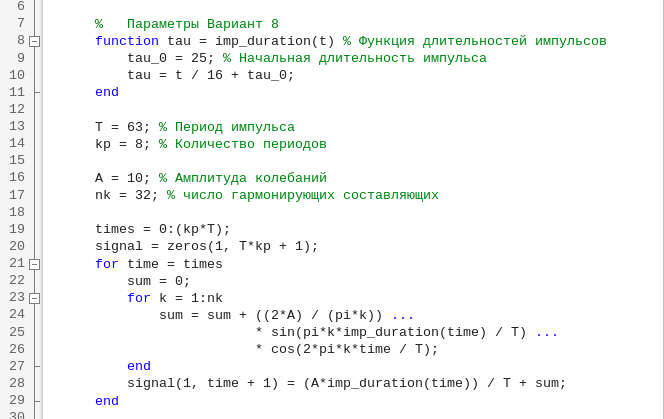
\includegraphics[width=\linewidth]{code_modelSig.png}
		\caption{Код генерации моделирующей функции}
	\end{figure}

  \subsection*{2.2 Генерация ШИМ-колебания}
  	Высокочастотные колебания:\\
  	$Un_t = A_Hcos(\omega_H t)$, где\\
  		$A_H$ - амплитуда ВЧ колебания ($A_H = 1$)\\
  		$\omega_H$ - угловая частота ($\omega_H = \frac{5 * 2\pi}{T}$)\\
  	
  	Итоговое колебание:\\
  	$Urez_t = s_t * Un_t$\\
  	
  	\begin{figure}[!h]
		\centering
		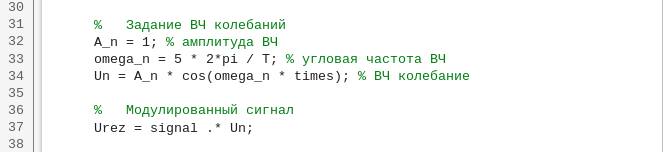
\includegraphics[width=\linewidth]{code_PW.png}
		\caption{Код генерации выходного сигнала}
	\end{figure}
 	
  \subsection*{2.3 Этапы отправки сигнала}
	\begin{figure}[!h]
		\centering
		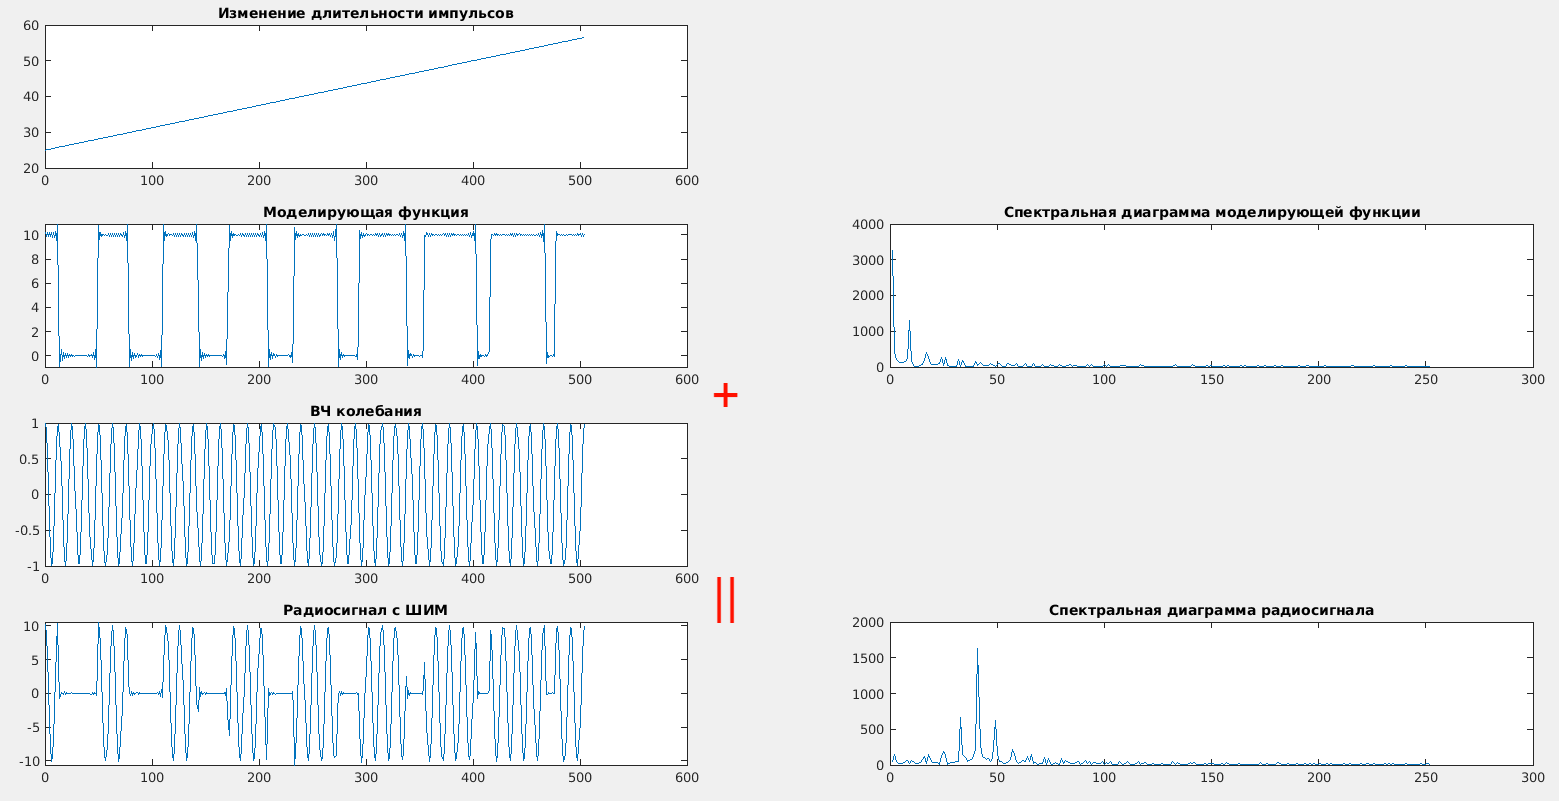
\includegraphics[width=\linewidth]{graph_output_colored.png}
		\caption{Генерация сигнала}
	\end{figure}

 
\newpage
 \section*{3. Приём ШИМ-сигнала}
 
  \subsection*{3.1 Обфускация сигнала}
  При передаче сигнала по каналу связи происходит некоторое его затухание и искажение помехами:\\
  $Ukr_t = (k * Urez_t) + Upom_t$, где \\
  k - коэффициент затухания полезного сигнала\\
  $Upom_t$ - мгновенные значения помех \\
  
  	\begin{figure}[!h]
		\centering
		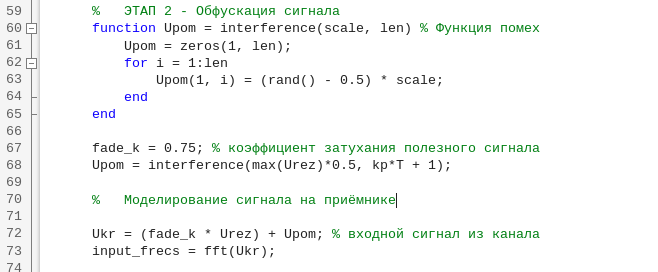
\includegraphics[width=\linewidth]{code_channel_sig.png}
		\caption{Код обфускации сигнала}
	\end{figure}
  
 
  \subsection*{3.2 Фильтрация сигнала от помех}
  	\begin{figure}[!h]
		\centering
		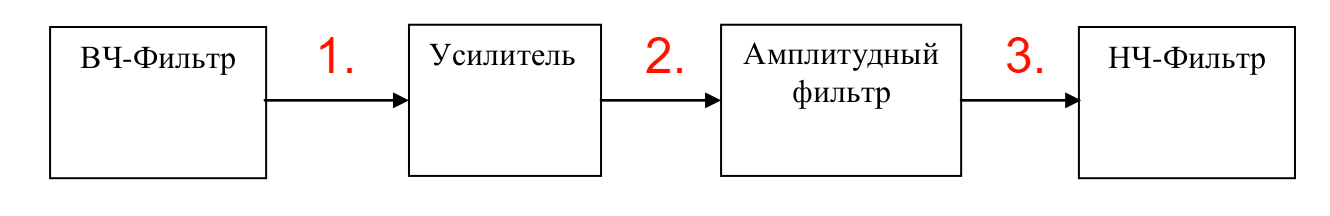
\includegraphics[width=1\linewidth]{filtering_scheme_colored.png}
		\caption{Схема фильтрации приемного устройства}
	\end{figure}
	
	Для фильтрации принимаемого сигнала последовательно используются:\\
	\begin{itemize}
		\item ВЧ-фильтр - \textbf{частотно}-избирательная фильтрация, в качестве оператора которой используется функция Хевисайда (1 если $x \geq \alpha$ 0 иначе)
		\item Усилитель - во \textbf{временной} области выражение напряжения имеет вид $Urez2_t = \frac{1}{k}Uk2_t$, где k - коэффициент полезного затухания сигнала
		\item НЧ-фильтр - фильтр нижних \text{частот}, частотная характеристика фильтра определяется выражением $k_t = \frac{1}{1+(\frac{t}{fn})^{2n}}$, где f - верхняя частота среза фильтра; n - порядок фильтра
	\end{itemize}
	
	Для перевода сигнала из временной области в частотную и обратно использовались функция быстрого преобразования Фурье и обратная к ней соответственно
	
	\begin{figure}[!h]
		\centering
		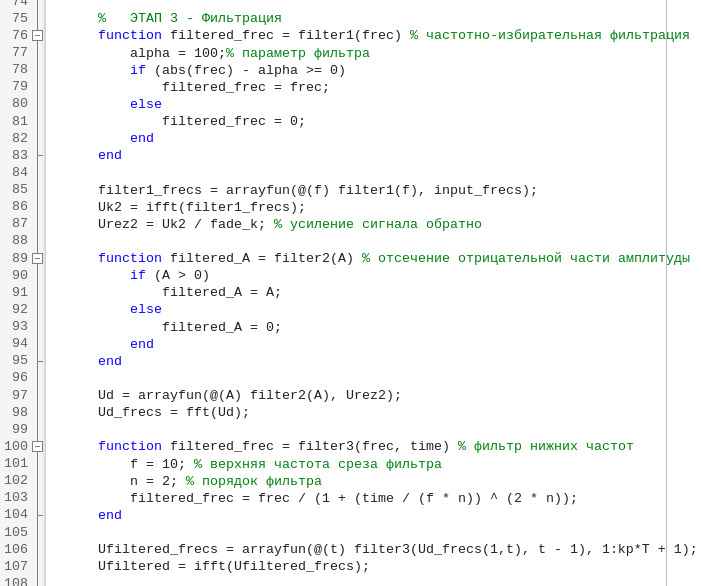
\includegraphics[width=0.92\linewidth]{code_filtering.png}
		\caption{Код этапов фильтрации сигнала}
	\end{figure}
	
 
  \subsection*{3.3 Этапы приёма сигнала}
  	\begin{figure}[!h]
		\centering
		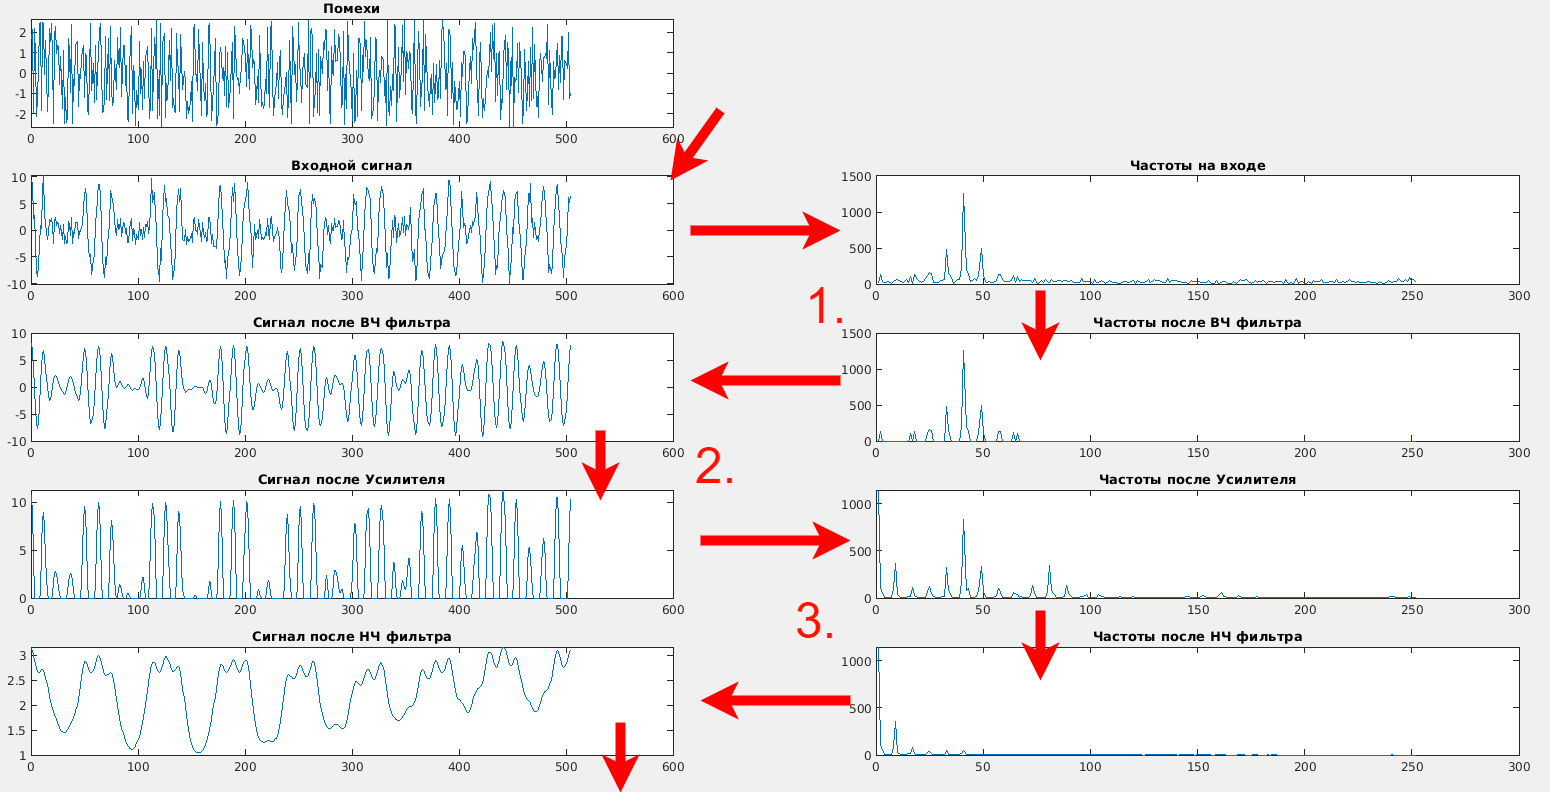
\includegraphics[width=1.2\linewidth]{graph_input_colored.png}
		\caption{Обработка сигнала}
	\end{figure}

\newpage
 \section*{4. Преобразование в импульсы}
 	После фильтрации была получена огибающая функция сигнала $h_t$, следующее выражение преобразует её в послеовательность униполярных прямоугольных импульсов:\\
 	$Udet_t = if (h_t > m, 1, 0)$, где m - эмпирически подобранный параметр, зависящий от формы $h_t$
 	
 	 \begin{figure}[!h]
		\centering
		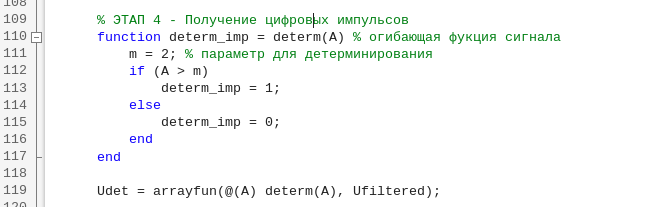
\includegraphics[width=\linewidth]{code_finalizing.png}
		\caption{Код преобразования в импульсы}
	\end{figure}
	
	\begin{figure}[!h]
		\centering
		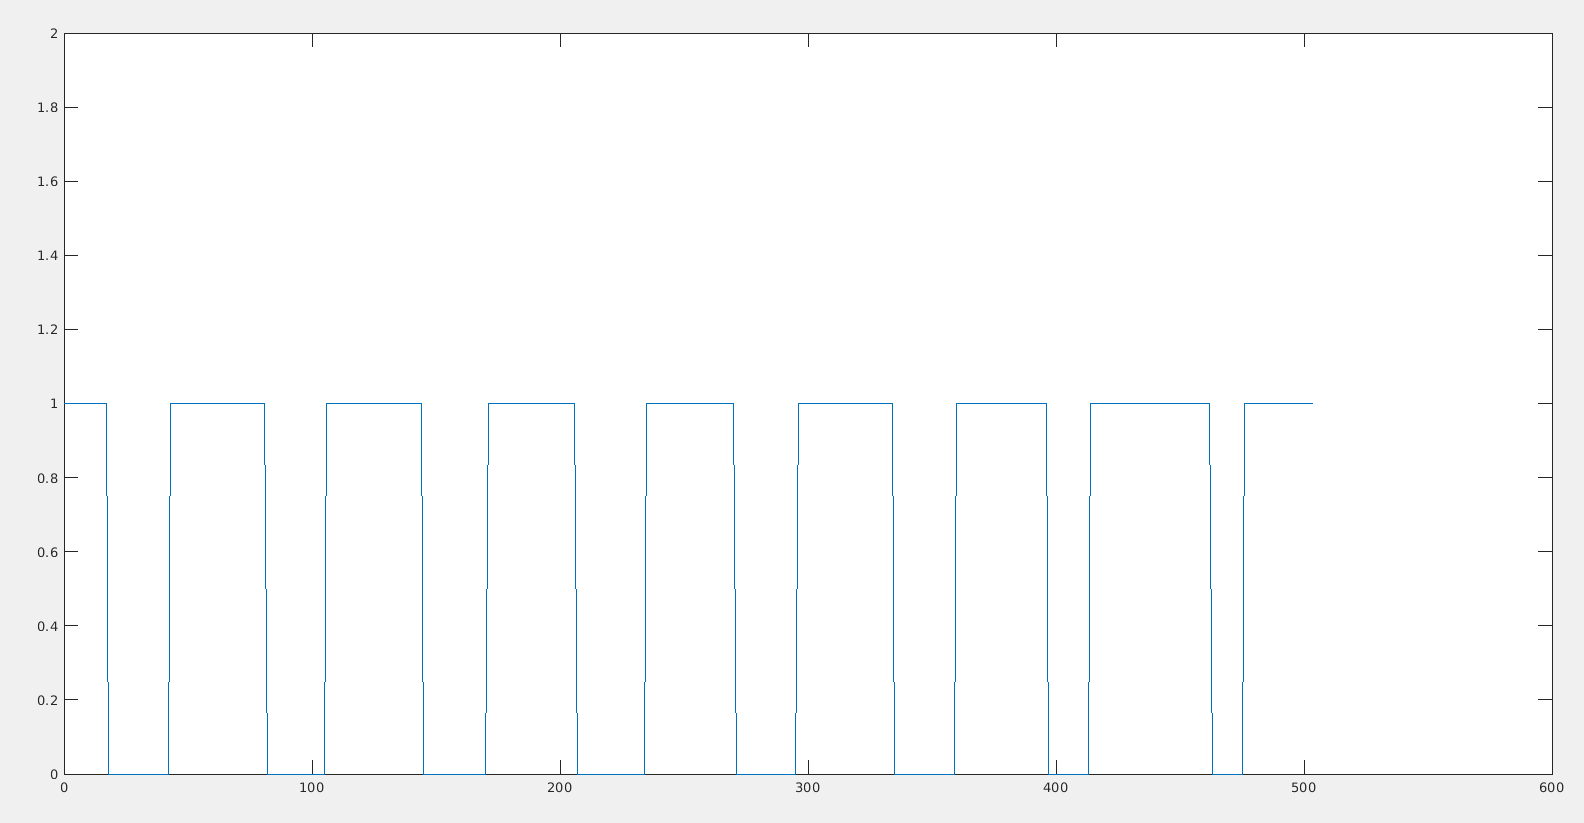
\includegraphics[width=0.75\linewidth]{final_signals.png}
		\caption{График полученных импульсов}
	\end{figure}
	
 	
	Полученные импульсы соответствуют изначально сформированной последовательности.
 

\end{document}